\documentclass[uplatex, titlepage, report]{jsbook}

%%%%%%%%%%%%%%%%%%%%%%%%%%%%%%%%%%%%%%%%%%%%%%%%%%%%
% パッケージはここに追加。
%1行目に何に使うか、2行目以降に使い方をコメントすること。
%%%%%%%%%%%%%%%%%%%%%%%%%%%%%%%%%%%%%%%%%%%%%%%%%%%%

%ベクトルの定義
\usepackage{bm} 
%一括コメントアウト
%\begin{comment}
\usepackage{comment}

%数学記号
%多数あるが、例えば\thereforeで'∴'(ゆえに)が出せる。
\usepackage{amssymb}

%行列、ベクトルなど
%\begin{pmatrix}…\end{pmatrix}。表と同じように区切り、改行する。縦ベクトルは1列の行列として表現。
\usepackage{amsmath}

%定理・補題・定義・証明
%\begin{theorem}, \begin{lemma}, \begin{definition}, \begin{proof}
\usepackage{amsthm}

%ブラケット記法
%\bra{a}, \ket{a}, \braket{a|H|a}。先頭を大文字にする(\Bra, \Ket, ...)と、
%中身の大きさに応じてブラケットの大きさも変わる。
\usepackage{braket}

%フォントの変更
%なし(自動)。
\usepackage{newpxtext, newpxmath}

%画像の挿入
%\includegraphics[width=***cm]{***.pdf}
\usepackage[dvipdfmx]{graphicx}

%文章を四角で囲む/左に線を引く
%\begin{oframed}、\begin{leftbar}など。
\usepackage{framed}

%図表を強制的にその場所に配置
%位置指定で[h]のかわりに[H]とする。これを使うと行間が不自然になる場合もある。
\usepackage{here}

%文字の色を変える
%\textcolor{red}{text}など。
\usepackage[dvipdfmx]{color} %jpg,png画像などの読み込みにはdvipdfmxオプションが必要。

%urlをそのまま記載できる
%\url{http://www.....}
\usepackage{url}

%urlやページへのリンク
%なし(自動)。
\usepackage[
    dvipdfmx,
    bookmarkstype=toc,
    setpagesize=false,
    colorlinks=true,
    urlcolor=black,
    linkcolor=black,
    citecolor=black,
    bookmarks=true,
    bookmarksopen=true,
    bookmarksnumbered=true]{hyperref}
    
%urlやページへのリンク(hyperrefを日本語環境で使用するのに必要)
%なし(自動)。
\usepackage{pxjahyper}

%著者をまとめて表示
%省略(rootでしか使用しないため)。
\usepackage{authblk}

%花文字
%\mathscr{A}
\usepackage{mathrsfs}

%化学式
%\ce{^3He},\ce{Na2SO3}
\usepackage[version=3]{mhchem}

%1つのキャプションに対して複数のサブキャプションをつける
%\includegraphics{figure1.pdf} \subcaption{caption1} includegraphics{figure2.pdf} \subcaption{caption2} \caption{caption}
\usepackage{subcaption}

%%%%%%%%%%%%%%%%%%%%%%%%%%%%%%%%%%%%%%%%%%%%%%%%%%%%
%マクロはここに追加。
%1行目に何に使うか、2行目以降に使い方をコメントすること。
%文書全体で使用するマクロのみここで定義。自分だけ使用する場合は、
%自分の文書を\begingroup - \endgroupもしくは{ }で囲み、その中で定義
%する。
%%%%%%%%%%%%%%%%%%%%%%%%%%%%%%%%%%%%%%%%%%%%%%%%%%%%

%等号の上下に文字列を表示。文字列の長さに応じて等号が伸縮。
%\xequal[下]{上}
\makeatletter
\newcommand{\xequal}[2][]{\ext@arrow 0055{\equalfill@}{#1}{#2}}
\def\equalfill@{\arrowfill@\Relbar\Relbar\Relbar}
\makeatother

%%%%%%%%%%%%%%%%%%%%%%%%%%%%%%%%%%%%%%%%%%%%%%%%%%%%
%スタイルの変更はここに追加。
%1行目に変更するスタイルをコメントすること。
%%%%%%%%%%%%%%%%%%%%%%%%%%%%%%%%%%%%%%%%%%%%%%%%%%%%
%脚注
\renewcommand{\thefootnote}{\arabic{footnote})}

%定理環境(amsthm)
\theoremstyle{definition}
\newtheorem{theorem}{定理}
\newtheorem{definition}[theorem]{定義}
\newtheorem{lemma}[theorem]{補題}
\renewcommand\proofname{\textbf{証明}}

%著者
\renewcommand\Authsep{\quad}
\renewcommand\Authands{\quad}

%もう少しまともなタイトルを考える
\title{KUANSにおける熱中性子を用いたスピン干渉実験}

\date{\vspace{3cm} 
\includegraphics[width=4cm]{logo_s.pdf}\\
\vspace{3.5cm} 提出年月\quad2017年3月}

\author[$\dagger$]{加須屋春樹}
\author[$\dagger$]{近藤寛記}
\author[$\dagger$]{鈴木一輝}
\author[$\dagger$]{武中亮}
\author[$\dagger$]{間宮章}
\author[$\dagger$]{藤井涼平}
%Bad practiceだが、こうするくらいしか思いつかない
\author[ ]{\\}

\affil[$\dagger$]{京都大学 理学部}
\author[ ]{\\}
\author[ ]{指導教員\quad}
\author[*]{成木恵 准教授}
\author[*]{菅沼秀夫 准教授}
\author[*]{国広悌二 教授}
\affil[*]{京都大学 理学研究科}
\begin{document}
\maketitle
\tableofcontents

%ここで文書をincludeします
\section*{概要}
\addcontentsline{toc}{section}{概要}
本実験の目的は中性子スピン状態の分解・再結合による中性子スピン干渉を確認することである。

KUANSではパルス型陽子加速器を用いて熱中性子を発生させている。
この中性子を偏極させ、スピンフリッパーを用いてスピンを分解する。
定磁場印加装置を利用し、スピンの向きによって位相のずれを生じさせ、
再びスピンフリッパーでスピンを再結合させることで干渉を起こさせる。

これにより、量子力学特有のスピン状態とその重ね合わせを実験的に確かめる。

\section{スーパーミラーによるスピンの選択}
\nocite{neutron_spin_optics}
この実験では、特定のスピンを持つ中性子を選択的に取り出す必要がある。この節では、そのために用いるスーパーミラーの原理について説明する。

\subsection{中性子の光学的性質}
\paragraph{屈折率}
中性子が物質中で感じるポテンシャルを$V$とすると、エネルギー保存から
\begin{align}
k^2-k'^2=2mV
\end{align}
となる。$k$は入射中性子の波数、$k'$は物質中での中性子の波数である。
屈折率の定義
\begin{align}
n=\frac{k'}{k}
\end{align}
から、中性子の物質中における屈折率は
\begin{align}
n^2=1-\frac{2mV}{k^2}\label{mirror_neutron_refindex}
\end{align}
となる。

\paragraph{全反射が起きる条件}\label{mirrir_perfect_reflection}
$n-1$が有限の値を持つことは、中性子が全反射しうることを意味する。全反射が起きるための角度の条件は、
臨界角
\begin{align}
\theta^*=\arccos{n}
\end{align}
を用いて
\begin{align}
n\leq\cos\theta^* \label{mirror_refindex_range}
\end{align}
となる。また、全反射が起きるための入射エネルギー$E$の条件は、(\ref{mirror_neutron_refindex}), (\ref{mirror_refindex_range})より
\begin{align}
&n^2=1-\frac{2mV}{k^2}\leq\cos^2\theta^*\\
&E\sin^2\theta\leq E\sin^2\theta^*=\frac{k^2}{2m}\sin^2\theta^*\leq V
\end{align}
となる。すなわち、臨界角以下で入射する時、エネルギーの``ミラーに対し垂直な成分''が$V$よりも小さければ、
全反射が起きることがわかる。

\subsection{磁性体単層膜によるスピンの選択}
磁性体の単層膜を利用することで、特定のスピンを持つ中性子を選択的に取り出すことができる。
中性子が単層膜中で受けるポテンシャルは、核力によるポテンシャル$V_\mathrm{n}$、単層膜中の磁束密度$B$を用いて
\begin{align}
V^{\pm}&=V_\mathrm{n}\pm|\mu_\mathrm{n}|B
\end{align}
となる。$\mu_\mathrm{n}|B|$の符号とスピンの向きの対応は磁場の向きによって決まるが、ここでは上向きスピンのときに正になるものとする。
すなわち、上向きスピンの中性子は$V^+$、下向きスピンの中性子は$V^-$を感じる。

\ref{mirrir_perfect_reflection}節で述べたように、入射中性子のエネルギーを$E$とすると、
\[
E\sin^2\theta\leq V
\]
のときに全反射が起きる。
$V^-< E\sin^2\theta\leq V^+$のエネルギーを持つ中性子をこの単層膜に入射させると、下向きスピンの中性子はほとんどが透過するが、
上向きスピンの中性子は全反射される。$V^+<E\sin^2\theta$の中性子が入射した場合は、上向き、下向き両方の粒子が
透過する確率を持つ。
そのため、透過した中性子には上向きスピンと下向きスピンの両方が含まれる。
$E\sin^2\theta\leq V^-$となるような低エネルギーの中性子は今回の実験では無視できるほど少ないため、
考えなくて良い。

\begin{figure}[h]
\centering
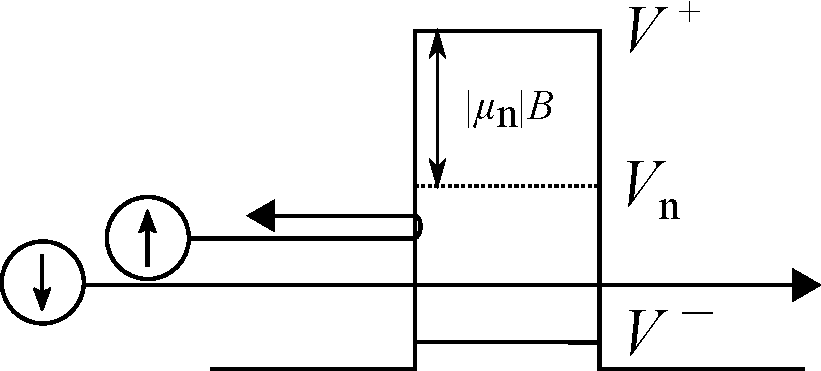
\includegraphics[width=8cm]{mirror/mono_mirror.pdf}
\caption{単層膜によるスピンの選択の原理。実際には、ポテンシャルは紙面奥に向かって2次元に広がっており、
中性子は臨界角以下で入射していることに注意。}
\end{figure}
このようにして、単層膜は上向きスピンの粒子のみを選択的に反射する。

\subsection{スーパーミラー}
\begin{figure}[H]
\centering
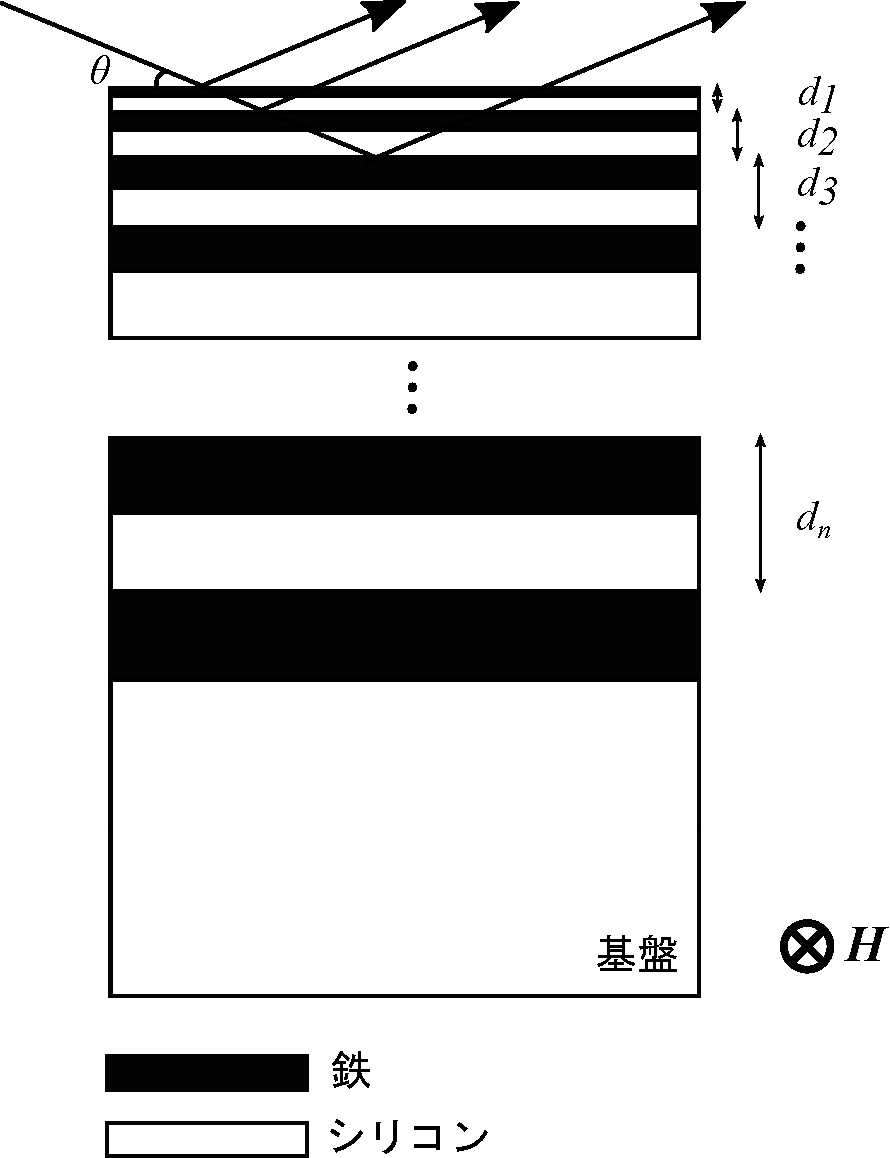
\includegraphics{mirror/super_mirror.pdf}
\caption{スーパーミラーの構造\cite{seki}\label{mirror_super_mirror}}
\end{figure}
\begin{figure}[h]
\centering
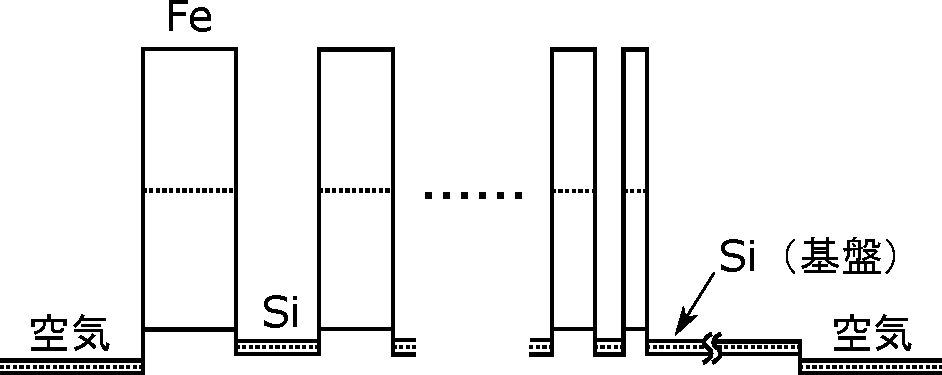
\includegraphics[width=9cm]{mirror/super_mirror_potential.pdf}
\caption{スーパーミラーのポテンシャル。破線は磁場によらない核力によるポテンシャル。実線(上)は上向きスピンの中性子が感じるポテンシャル。
実線(下)は下向きスピンの中性子が感じるポテンシャル。空気やシリコンの透磁率は小さいため、全体に磁場をかけても
ポテンシャルはほとんど影響を受けない。}
\end{figure}
図\ref{mirror_super_mirror}のように膜厚を少しずつ変えた多層膜を使うことで、
単層膜よりも高いエネルギーの中性子を反射するミラーを作ることができる。
これをスーパーミラーと呼ぶ。

\paragraph{Bragg反射による偏極}
$E\sin^2\theta\leq V^+$の中性子は多層膜の表面で全反射されるが、$V^+<E\sin^2\theta$の中性子は多層膜の内部に侵入する。
多層膜の膜間隔を$d$とすると、侵入した中性子はBragg条件
\begin{align}
2d\sin\theta=\lambda
\end{align}
を満たす場合に反射波が強め合う。$\lambda$は中性子の物質波の波長で、
$\lambda=2\pi/k$の関係にある。

$d$を少しずつ変えることで、$V^+<E\sin^2\theta$の様々なエネルギーを持つ上向きスピンの中性子がBragg反射される。
下向きスピンの中性子もわずかに反射されるが、その数は少なく、無視できる。
こうすることで、単層膜に比べより広いエネルギーの中性子のスピンを偏極することができる。

\def\vector#1{\mbox{\boldmath $#1$}}
\section{実験原理}
領域Ⅰから、
\begin{align}
{\psi}_{Ⅰ}(x,t)=
\begin{pmatrix}
e^{-iw_{z}x/v} \\
0
\end{pmatrix}
e^{ik_{0}x}e^{-iw_{0}t}
\end{align}
のような波動関数で表される粒子が、領域Ⅶでどのような状態になるのかを考える。

領域Ⅱにおける磁場は
\begin{align}
\bm{B}=B_{r}\cos(w_{s}t)\bm{\hat{x}}+B_{r}\sin(w_{s}t)\bm{\hat{y}}+B_{z}\bm{\hat{z}}
\end{align}
とする。
\begin{align}
w_{r}=|{\mu}B_{r}|
\end{align}
\begin{align}
w_{z}=|{\mu}B_{z}|
\end{align}
とする。この時、領域Ⅱにおけるシュレディンガー方程式は
\begin{align}
i\frac{\partial {\psi}_{Ⅱ}(x,t)}{\partial t}=\left(-\frac{1}{2m}\frac{\partial^2}{\partial x^2}+w_{r}\cos(w_{s}t){\sigma}_{x}+w_{r}\sin(w_{s}t){\sigma}_{y}+{\hbar}w_{z}{\sigma}_{z}\right){\psi}_{Ⅱ}(x,t)
\end{align}
と書ける。ここで、
\begin{align}
w_{r}\cos(w_{s}t){\sigma}_{x}+w_{r}\sin(w_{s}t){\sigma}_{y}+w_{z}{\sigma}_{z}=
\begin{pmatrix}
w_{z} &w_{r}e^{-iw_{s}t} \\
w_{r}e^{iw_{s}t} &-w_{z}
\end{pmatrix}
\end{align}
$と書ける。角速度w_{s}でz軸の周りに回転するユニタリー変換$
\begin{align}
U_{T}=\exp(iw_{s}t{\sigma}_{z})=
\begin{pmatrix}
e^{iw_{s}t} &0 \\
0 &e^{-iw_{s}t}
\end{pmatrix}
\end{align}
をもちいて
\begin{align}
U_{T}\begin{pmatrix}
w_{z} &w_{r}e^{-iw_{s}t} \\
w_{r}e^{iw_{s}t} &-w_{z}
\end{pmatrix}U_{T}^{\dagger}=
\begin{pmatrix}
w_{z} &w_{r} \\
w_{r} &-w_{z}
\end{pmatrix}
\end{align}
が成り立つ。
\begin{align}
{\psi}_{R}(x,t)=U_{T}{\psi}(x,t)
\end{align}
$とすると{\psi}_{R}(x,t)の満たすシュレディンガー方程式は$
\begin{align}
i\frac{\partial {\psi}_{R}(x,t)}{\partial t}=\left(-\frac{1}{2m}\frac{\partial^2}{\partial x^2}+w_{r}{\sigma}_{x}+\left(w_{z}-\frac{1}{2}w_{s}\right){\sigma}_{z}\right){\psi}_{R}(x,t)
\end{align}
となる。いま、共鳴条件
\begin{align}
{\epsilon}=\frac{1}{2}w_{s}-w_{z}=0
\end{align}
が成り立っているとする。この時、シュレディンガー方程式は
\begin{align}
i\frac{\partial {\psi}_{R}(x,t)}{\partial t}=\left(-\frac{1}{2m}\frac{\partial^2}{\partial x^2}+w_{r}{\sigma}_{x}\right){\psi}_{R}(x,t)
\end{align}
いま、
\begin{align}
U_{D}=\exp(i{\pi}{\sigma}_{y}/4)=
\begin{pmatrix}
1/\sqrt{2} &1/\sqrt{2} \\
-1/\sqrt{2} &1/\sqrt{2}
\end{pmatrix}
\end{align}
というユニタリー変換を用いると、
\begin{align}
U_{D}{\sigma}_{x}U_{D}^{\dagger}={\sigma}_{z}
\end{align}
が成り立つ。
\begin{align}
{\psi}_{D}(x,t)=U_{D}{\psi}_{R}(x,t)
\end{align}
$とすると、{\psi}_{D}(x,t)の満たすシュレーディンガー方程式は$
\begin{align}
i\frac{\partial {\psi}_{D}(x,t)}{\partial t}=\left(-\frac{1}{2m}\frac{\partial^2}{\partial x^2}+w_{r}{\sigma}_{z}\right){\psi}_{D}(x,t)
\end{align}
$この方程式の解のうち、エネルギー固有値がE_{n}=w_{n}であるものは$
\begin{align}
{\psi}_{D}(x,t) =
\begin{pmatrix}
A_{n}^{+}e^{ik_{n}^{+}x}+B_{n}^{+}e^{-ik_{n}^{+}x}  \\
A_{n}^{-}e^{ik_{n}^{-}x}+B_{n}^{-}e^{-ik_{n}^{-}x}
\end{pmatrix}
e^{-iw_{n}t}
\end{align}
ここで、
\begin{align}
\frac{{k_{n}^{\pm}}^2}{2m}{\pm}w_{r}=E_{n}
\end{align}
が成り立つ。ゆえに、領域Ⅱにおける波動関数は
\begin{align}
{\psi}_{Ⅱ}(x,t)=U_{T}^{\dagger}U_{D}^{\dagger}{\psi}_{D}(x,t)=\frac{1}{\sqrt{2}}
\begin{pmatrix}
\left[(A_{n}^{+}e^{ik_{n}^{+}x}+B_{n}^{+}e^{-ik_{n}^{+}x})+(A_{n}^{-}e^{ik_{n}^{-}x}+B_{n}^{-}e^{-ik_{n}^{-}x})\right]e^{-i(w_{n}+w_{s}/2)t} \\
\left[(A_{n}^{+}e^{ik_{n}^{+}x}+B_{n}^{+}e^{-ik_{n}^{+}x})-(A_{n}^{-}e^{ik_{n}^{-}x}+B_{n}^{-}e^{-ik_{n}^{-}x})\right]e^{-i(w_{n}-w_{s}/2)t}
\end{pmatrix}
\end{align}

いま、入射波、すなわち領域Ⅰにおける波動関数を
\begin{align}
{\psi}_{Ⅰ}(x,t)=
\begin{pmatrix}
e^{-iw_{z}x/v} \\
0
\end{pmatrix}
e^{ik_{0}x}e^{-iw_{0}t}
\end{align}
$とする。ここで、v={k_{0}}/{m}であり、$
\begin{align}
\frac{k_{0}^2}{2m}=E_{0}=w_{0}
\end{align}
$が成り立つ。x=0における接続条件により、以下の4つの式が任意のtについて成り立つ。$
\begin{align}
e^{-iw_{0}t}=\left[(A_{n}^{+}+B_{n}^{+})+(A_{n}^{-}+B_{n}^{-})\right]e^{-i(w_{n}+w_{s}/2)t}
\end{align}
\begin{align}
0=\left[(A_{n}^{+}+B_{n}^{+})-(A_{n}^{-}+B_{n}^{-})\right]e^{-i(w_{n}-w_{s}/2)t}
\end{align}
\begin{align}
(k_{0}-w_{z}/v)e^{-iw_{0}t}=\left[k_{n}^{+}(A_{n}^{+}-B_{n}^{+})+k_{n}^{-}(A_{n}^{-}-B_{n}^{-})\right]e^{-i(w_{n}+w_{s}/2)t}
\end{align}
\begin{align}
0=\left[k_{n}^{+}(A_{n}^{+}-B_{n}^{+})-k_{n}^{-}(A_{n}^{-}-B_{n}^{-})\right]e^{-i(w_{n}-w_{s}/2)t}
\end{align}
これにより、
\begin{align}
w_{n}=w_{0}-w_{s}/2
\end{align}
$を満たすn以外のnについて$
\begin{align}
A_{n}^{+}=B_{n}^{+}=A_{n}^{-}=B_{n}^{-}=0
\end{align}
となる。また、
\begin{align}
w_{n}=w_{0}-w_{s}/2
\end{align}
$を満たすnを1とすると、A_{1}^{\pm},B_{1}^{\pm}は0ではない。以上から、$
\begin{align}
{\psi}_{Ⅱ}(x,t) \notag
=&\frac{1}{\sqrt{2}}
\begin{pmatrix}
\left[(A_{1}^{+}e^{ik_{1}^{+}x}+B_{1}^{+}e^{-ik_{1}^{+}x})+(A_{1}^{-}e^{ik_{1}^{-}x}+B_{1}^{-}e^{-ik_{1}^{-}x})\right]e^{-i(w_{1}+w_{s}/2)t} \\
\left[(A_{1}^{+}e^{ik_{1}^{+}x}+B_{1}^{+}e^{-ik_{1}^{+}x})-(A_{1}^{-}e^{ik_{1}^{-}x}+B_{1}^{-}e^{-ik_{1}^{-}x})\right]e^{-i(w_{1}-w_{s}/2)t}
\end{pmatrix}\\
=&\begin{pmatrix}
\left[(A_{1}^{+}e^{ik_{1}^{+}x}+B_{1}^{+}e^{-ik_{1}^{+}x})+(A_{1}^{-}e^{ik_{1}^{-}x}+B_{1}^{-}e^{-ik_{1}^{-}x})\right]e^{-iw_{0}t} \\
\left[(A_{1}^{+}e^{ik_{1}^{+}x}+B_{1}^{+}e^{-ik_{1}^{+}x})-(A_{1}^{-}e^{ik_{1}^{-}x}+B_{1}^{-}e^{-ik_{1}^{-}x})\right]e^{-i(w_{0}-w_{s})t}
\end{pmatrix}
\end{align}
$透過波、すなわち領域Ⅲにおける波動関数のうち、エネルギー固有値がE_{n}であるものは以下のようなものである。$
\begin{align}
{\psi}_{Ⅲ}(x,t)=
\begin{pmatrix}
C_{n}^{+}e^{iK_{n}^{+}x} \\
C_{n}^{-}e^{iK_{n}^{-}x}
\end{pmatrix}
e^{-iw_{n}t}
\end{align}
ここで
\begin{align}
\frac{{K_{n}^{\pm}}^2}{2m}{\pm}w_{z}=w_{n}
\end{align}
$が成り立つ。x=dにおける接続より、以下の4つの式が任意のtについて成り立つ。$
\begin{align}
C_{n}^{+}e^{iK_{n}^{+}d}e^{-iw_{n}t}=\left[(A_{1}^{+}e^{ik_{1}^{+}d}+B_{1}^{+}e^{-ik_{1}^{+}d})+(A_{1}^{-}e^{ik_{1}^{-}d}+B_{1}^{-}e^{-ik_{1}^{-}d})\right]e^{-iw_{0}t}
\end{align}
\begin{align}
C_{n}^{-}e^{iK_{n}^{-}d}e^{-iw_{n}t}=\left[(A_{1}^{+}e^{ik_{1}^{+}d}+B_{1}^{+}e^{-ik_{1}^{+}d})-(A_{1}^{-}e^{ik_{1}^{-}d}+B_{1}^{-}e^{-ik_{1}^{-}d})\right]e^{-i(w_{0}-w_{s})t}
\end{align}
\begin{align}
iK_{n}^{+}C_{n}^{+}e^{iK_{n}^{+}d}e^{-iw_{n}t}=\left[ik_{1}^{+}(A_{1}^{+}e^{ik_{1}^{+}d}-B_{1}^{+}e^{-ik_{1}^{+}d})+ik_{1}^{-}(A_{1}^{-}e^{ik_{1}^{-}d}-B_{1}^{-}e^{-ik_{1}^{-}d})\right]e^{-iw_{0}t}
\end{align}
\begin{align}
iK_{n}^{-}C_{n}^{-}e^{iK_{n}^{-}d}e^{-iw_{n}t}=\left[ik_{1}^{+}(A_{1}^{+}e^{ik_{1}^{+}d}-B_{1}^{+}e^{-ik_{1}^{+}d})-ik_{1}^{-}(A_{1}^{-}e^{ik_{1}^{-}d}-B_{1}^{-}e^{-ik_{1}^{-}d})\right]e^{-i(w_{0}-w_{s})t}
\end{align}
$いま、w_{n}=w_{0}でもw_{n}=w_{0}-w_{s}でもないnについては$
\begin{align}
C_{n}^{+}=C_{n}^{-}=0
\end{align}
が成り立つ。ゆえに、
\begin{align}
w_{2}=w_{0}-w_{s}
\end{align}
$とすると、残るのはnが0と2だけで、さらに$
\begin{align}
C_{0}^{-}=C_{2}^{+}=0
\end{align}
透過波はこれらを重ね合わせた
\begin{align}
{\psi}_{Ⅲ}(x,t)=
\begin{pmatrix}
C_{0}^{+}e^{iK_{0}^{+}x} \\
0
\end{pmatrix}
e^{-iw_{0}t}+
\begin{pmatrix}
0 \\
C_{2}^{-}e^{iK_{2}^{-}x}
\end{pmatrix}
e^{-iw_{2}t}
=\begin{pmatrix}
C_{0}^{+}e^{iK_{0}^{+}x}e^{-iw_{0}t} \\
C_{2}^{-}e^{iK_{2}^{-}x}e^{-i(w_{0}-w_{s})t}
\end{pmatrix}
\end{align}
である。ここで、
\begin{align}
\frac{{K_{n}^{\pm}}^2}{2m}{\pm}w_{z}=w_{n}
\end{align}
により、
\begin{align}
\frac{{K_{0}^{+}}^2}{2m}+w_{z}=w_{0}
\end{align}
\begin{align}
\frac{{K_{2}^{-}}^2}{2m}-w_{z}=w_{0}-w_{s}
\end{align}
よって
\begin{align}
K_{0}^{+}=\sqrt{2m(w_{0}-w_{z})}{\simeq}k_{0}-w_{z}/v
\end{align}
\begin{align}
K_{2}^{-}=\sqrt{2m((w_{0}-w_{s})+w_{z})}{\simeq}k_{0}+(w_{z}-w_{s})/v
\end{align}
よって
\begin{align}
{\psi}_{Ⅲ}(x,t)=
\begin{pmatrix}
C_{0}^{+}e^{iK_{0}^{+}x}e^{-iw_{0}t} \\
C_{2}^{-}e^{iK_{2}^{-}x}e^{-i(w_{0}-w_{s})t}
\end{pmatrix}
{\simeq}
\begin{pmatrix}
C_{0}^{+}e^{i(k_{0}-w_{z}/v)x}e^{-iw_{0}t} \\
C_{2}^{-}e^{i(k_{0}+(w_{z}-w_{s})/v)x}e^{-i(w_{0}-w_{s})t}
\end{pmatrix}=
\begin{pmatrix}
C_{0}^{+}e^{i(-w_{z}/v)x} \\
C_{2}^{-}e^{i((w_{z}-w_{s})/v)x}e^{iw_{s}t}
\end{pmatrix}
e^{ik_{0}x}e^{-iw_{0}t}
\end{align}
ここで、共鳴条件
\begin{align}
w_{s}=2w_{z}
\end{align}
により、
\begin{align}
{\psi}_{Ⅲ}(x,t)=& \notag
\begin{pmatrix}
C_{0}^{+}e^{i(-w_{z}/v)x} \\
C_{2}^{-}e^{i(-w_{z}/v)x}e^{iw_{s}t}
\end{pmatrix}
e^{ik_{0}x}e^{-iw_{0}t}\\ \notag
=&\begin{pmatrix}
C_{0}^{+} \\
C_{2}^{-}e^{iw_{s}t}
\end{pmatrix}
e^{-iw_{z}/vx}e^{ik_{0}x}e^{-iw_{0}t}\\ 
=&\begin{pmatrix}
\cos(w_{r}d/v) \\
-i\sin(w_{r}d/v)e^{iw_{s}t}
\end{pmatrix}
e^{-iw_{z}/vx}e^{ik_{0}x}e^{-iw_{0}t}  
=&\begin{pmatrix}
\cos(w_{r}d/v)e^{i(k_{0}-w_{z}/v)x}e^{-iw_{0}t} \\
-i\sin(w_{r}d/v)e^{i(k_{0}-w_{z}/v)x}e^{-i(w_{0}-w_{s})t} 
\end{pmatrix}
\end{align}

$領域ⅢとⅣの境界x=l_{1}における波動関数は$
\begin{align}
{\psi}_{Ⅲ}(x=l_{1},t)=
\begin{pmatrix}
\cos(w_{r}d/v)e^{i(k_{0}-w_{z}/v)l_{1}}e^{-iw_{0}t} \\
-i\sin(w_{r}d/v)e^{i(k_{0}-w_{z}/v)l_{1}}e^{-i(w_{0}-w_{s})t}
\end{pmatrix}
\end{align}
$領域Ⅳにおける磁場をB={w}/{\mu}とすると、この領域ではスピン上成分が波数$
\begin{align}
k_{0}-w/v
\end{align}
スピン下成分が波数
\begin{align}
k_{0}-(w-w_{s})/v
\end{align}
で進んでいくので、領域Ⅳにおける波動関数は、
\begin{align}
{\psi}_{Ⅳ}(x,t)=
\begin{pmatrix}
\cos(w_{r}d/v)e^{i(k_{0}-w_{z}/v)l_{1}}e^{i(k_{0}-w/v)(x-l_{1})}e^{-iw_{0}t} \\
-i\sin(w_{r}d/v)e^{i(k_{0}-w_{z}/v)l_{1}}e^{i(k_{0}-(w-w_{s})/v)(x-l_{1})}e^{-i(w_{0}-w_{s})t}
\end{pmatrix}
\end{align}

領域Ⅴでは、両成分とも波数
\begin{align}
k_{0}-w_{z}/v
\end{align}
で進んでいくので、領域Ⅴにおける波動関数は
\begin{align}
{\psi}_{Ⅴ}(x,t)=
\begin{pmatrix}
\cos(w_{r}d/v)e^{i(k_{0}-w_{z}/v)l_{1}}e^{i(k_{0}-w/v)(l_{2}-l_{1})}e^{i(k_{0}-w_{z}/v)(x-l_{2})}e^{-iw_{0}t} \\
-i\sin(w_{r}d/v)e^{i(k_{0}-w_{z}/v)l_{1}}e^{i(k_{0}-(w-w_{s})/v)(l_{2}-l_{1})}e^{i(k_{0}-w_{z}/v)(x-l_{2})}e^{-i(w_{0}-w_{s})t}
\end{pmatrix}
\end{align}

$領域ⅤとⅥの境界x=l_{3}における波動関数は$
\begin{align}
{\psi}_{Ⅴ}(x=l_{3},t)=
\begin{pmatrix}
{\alpha}e^{-iw_{0}t} \\
{\beta}e^{-i(w_{0}-w_{s})t}
\end{pmatrix}
\end{align}
ここで、
\begin{align}
{\alpha}=\cos\left(w_{r}d/v\right)e^{i(k_{0}-w_{z}/v)l_{1}}e^{i\left(k_{0}-w/v\right)(l_{2}-l_{1})}e^{i\left(k_{0}-w_{z}/v\right)(l_{3}-l_{2})}
\end{align}
\begin{align}
{\beta}=i\sin\left(w_{r}d/v\right)e^{i(k_{0}-w_{z}/v)l_{1}}e^{i\left(k_{0}-(w-w_{s})/v\right)(l_{2}-l_{1})}e^{i\left(k_{0}-w_{z}/v\right)(l_{3}-l_{2})}
\end{align}
$領域Ⅵにおける波動関数のうち、エネルギーがE_{n}であるものは$
\begin{align}
{\psi}_{Ⅵ}(x,t)=
\begin{pmatrix}
(D_{n}^{+}e^{ik_{n}^{+}x}+D_{n}^{-}e^{ik_{n}^{-}x} )e^{-i(w_{n}+w_{s}/2)t}\\
(D_{n}^{+}e^{ik_{n}^{+}x}-D_{n}^{-}e^{ik_{n}^{-}x} )e^{-i(w_{n}-w_{s}/2)t}
\end{pmatrix}
\end{align}
である。ここで、
\begin{align}
\frac{{k_{n}^{\pm}}^2}{2m}{\pm}w_{r}=w_{n}
\end{align}
$が成り立つ。x=l_{3}における接続により$
\begin{align}
{\alpha}e^{-iw_{0}t}=\left(D_{n}^{+}e^{ik_{n}^{+}l_{3}}+D_{n}^{-}e^{ik_{n}^{-}l_{3}}\right)e^{-i\left(w_{n}+w_{s}/2\right)t}
\end{align}
\begin{align}
{\beta}e^{-i(w_{0}-w_{s})t}=\left(D_{n}^{+}e^{ik_{n}^{+}l_{3}}-D_{n}^{-}e^{ik_{n}^{-}l_{3}}\right)e^{-i\left(w_{n}-w_{s}/2\right)t}
\end{align}
すると
\begin{align}
w_{2}=w_{0}-w_{s}/2
\end{align}
$として、n=2のもの以外は0になる。$
\begin{align}
{\alpha}=\left(D_{2}^{+}e^{ik_{2}^{+}l_{3}}+D_{2}^{-}e^{ik_{2}^{-}l_{3}}\right)
\end{align}
\begin{align}
{\beta}=\left(D_{2}^{+}e^{ik_{2}^{+}l_{3}}-D_{2}^{-}e^{ik_{2}^{-}l_{3}}\right)
\end{align}
よって
\begin{align}
D_{2}^{+}=\frac{1}{2}e^{-ik_{2}^{+}l_{3}}({\alpha}+{\beta})
\end{align}
\begin{align}
D_{2}^{-}=\frac{1}{2}e^{-ik_{2}^{-}l_{3}}({\alpha}-{\beta})
\end{align}
ゆえに、領域Ⅵにおける波動関数は
\begin{align}
{\psi}_{Ⅵ}(x,t)=\frac{1}{2}
\begin{pmatrix}
\left(({\alpha}+{\beta})e^{ik_{2}^{+}(x-l_{3})}+({\alpha}-{\beta})e^{ik_{2}^{-}(x-l_{3})}\right)e^{-iw_{0}t}\\
\left(({\alpha}+{\beta})e^{ik_{2}^{+}(x-l_{3})}-({\alpha}-{\beta})e^{ik_{2}^{-}(x-l_{3})}\right)e^{-i(w_{0}-w_{s})t}
\end{pmatrix}
\end{align}

領域Ⅶでは両成分とも波数
\begin{align}
k_{0}-w_{z}/v
\end{align}
で進んでいくので、波動関数は
\begin{align}
{\psi}_{Ⅶ}(x,t)=\frac{1}{2}
\begin{pmatrix}
\left(({\alpha}+{\beta})e^{ik_{2}^{+}(l_{4}-l_{3})}+({\alpha}-{\beta})e^{ik_{2}^{-}(l_{4}-l_{3})}\right)e^{i(k_{0}-w_{z}/v)(x-l_{4})}e^{-iw_{0}t}\\
\left(({\alpha}+{\beta})e^{ik_{2}^{+}(l_{4}-l_{3})}-({\alpha}-{\beta})e^{ik_{2}^{-}(l_{4}-l_{3})}\right)e^{i(k_{0}-w_{z}/v)(x-l_{4})}e^{-i(w_{0}-w_{s})t}
\end{pmatrix}
\end{align}
スピン上成分の絶対値の2乗は
\begin{align}
\left|({\psi}_{Ⅶ}(x,t))_{+}\right|^2=\frac{1}{4}\left|({\alpha}+{\beta})e^{ik_{2}^{+}(l_{4}-l_{3})}+({\alpha}-{\beta})e^{ik_{2}^{-}(l_{4}-l_{3})}\right|^2
\end{align}
ここで、
\begin{align}
\frac{{k_{n}^{\pm}}^2}{2m}{\pm}w_{r}=w_{n}
\end{align}
により、
\begin{align}
\frac{{k_{2}^{\pm}}^2}{2m}{\pm}w_{r}=w_{2}=w_{0}-w_{s}/2=w_{0}-w_{z}
\end{align}
\begin{align}
k_{2}^{\pm}{\simeq}k_{0}-\frac{w_{z}{\pm}w_{r}}{v}
\end{align}
よって
\begin{align}
|({\psi}_{Ⅶ}(x,t))_{+}|^2 \notag
=&\frac{1}{4}\left|({\alpha}+{\beta})e^{-iw_{r}/v(l_{4}-l_{3})}+({\alpha}-{\beta})e^{iw_{r}/v(l_{4}-l_{3})}\right|^2\\ \notag
=&\left|{\alpha}\cos\left(\frac{w_{r}}{v}(l_{4}-l_{3})\right)-i{\beta}\sin\left(\frac{w_{r}}{v}(l_{4}-l_{3})\right)\right|^2\\ \notag
=&\left|e^{i(k_{0}-w/v)(l_{2}-l_{1})}\cos\left(\frac{w_{r}}{v}d\right)\cos\left(\frac{w_{r}}{v}(l_{4}-l_{3})\right)\right. \\
\left. +e^{i(k_{0}+(w-w_{s})/v)(l_{2}-l_{1})}\sin\left(\frac{w_{r}}{v}d\right)\sin\left(\frac{w_{r}}{v}(l_{4}-l_{3})\right)\right|^2
\end{align}
$ゆえに、領域Ⅳにおける磁場Bの大きさを変えながらビームの下流でスピン上成分の粒子の数を測定すると、干渉が観測できる。$







\section{検出器}
中性子は電荷をもたないため、その検出は強い相互作用を通じて行われる。強い相互作用による反応で生じた荷電粒子を検出することで、間接的に中性子を検出する。検出に利用する反応は検出する中性子のエネルギーによって様々であるが、熱中性子($\sim 25$ meV)の場合、次のような中性子捕獲反応が主に利用される:
\begin{align}
&\ce{^3He} + \ce{n} \to \ce{^3H}+\ce{p} + 0.705 \mathrm{MeV} \label{Kasuya_3He} \\
&\ce{^6Li} + \ce{n} \to \ce{^3H}+\ce{^4He}+4.78 \mathrm{MeV} \label{Kasuya_6Li}
\end{align}

\subsection{$\ce{^3He}$ガスを充填した比例計数管}
今回の実験では入射する中性子の時間情報と個数を知る必要がある。そこで入射粒子の数を1つずつ数える微分型の検出器として、$\ce{^3He}$ガスを充填した比例計数管を用いた。

\paragraph{検出原理}
検出には(\ref{Kasuya_3He})の反応が利用される。反応で生じた荷電粒子が気体中を進むと、軌道上の気体分子が電離してイオン・電子対が生じる。電場をかけてそれらを集めることで、信号として読み取ることができる。エネルギー25meVの中性子に対する$\ce{^3He}$原子核の断面積は$5333$barn[]であり、低エネルギーでこの断面積は中性子の速度に反比例することが知られている[]ため、エネルギー$E$(meV)の中性子に対する$\ce{^3He}$原子核の断面積は$\sigma(E)=5333\sqrt{25/E}$(barn)となる。これは気体の中では非常に大きく、効率よく中性子の数を数えることができる。

\paragraph{検出器の仕組み}
円筒形の容器の中に$\ce{^3He}$ガスが封入されており、高電圧がかけられた中心のワイヤと接地された容器の内壁がそれぞれ陽極と陰極として機能する。$\ce{^3He}$ガスは(\ref{Kasuya_3He})の反応によって荷電粒子を発生させる中性子有感物質であると共に、この荷電粒子によって電離して信号を増幅させる被電離気体の役割を果たす。

\begin{figure}[h]
\begin{minipage}{0.5\hsize}
\begin{center}
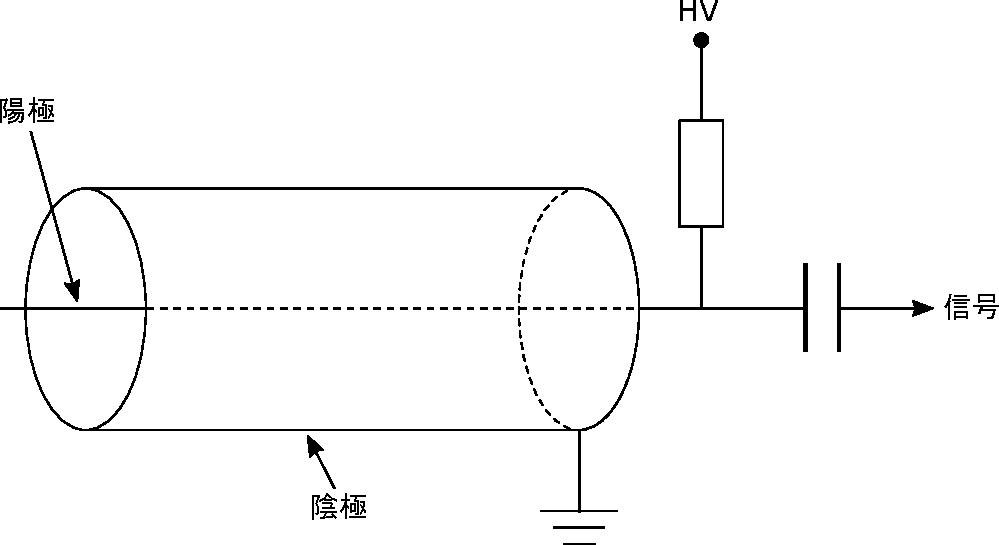
\includegraphics[width=6.5cm]{detector/detector_fig1.pdf}
\caption{比例計数管写真}
\end{center}
\end{minipage}
\begin{minipage}{0.5\hsize}
\begin{center}
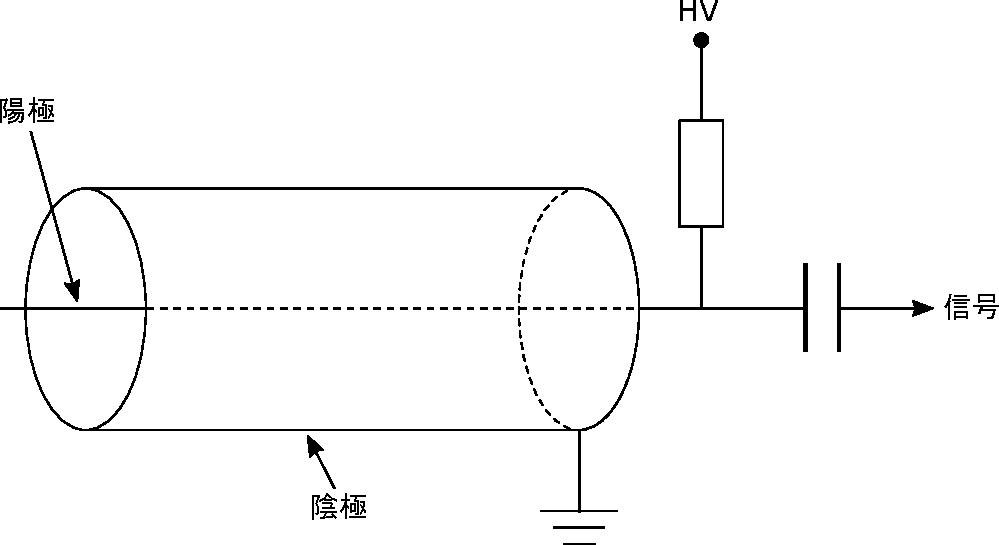
\includegraphics[width=6.5cm]{detector/detector_fig1.pdf}
\caption{比例計数管模式図}
\end{center}
\end{minipage}
\end{figure}

\subsection{RPMT検出器}
予備実験では入射する中性子の2次元的な位置情報を知る必要がある。そこで2次元位置感度型検出器として、RPMT検出器を用いた。

\paragraph{検出原理}
検出には(\ref{Kasuya_6Li})の反応が利用される。反応で生じた荷電粒子によってシンチレータ中の原子や分子が励起され、下の準位に戻る際に光が放出される(シンチレーション光)。生じた光は光電子増倍管で増幅され信号として取り出される。RPMTではシンチレータに$\ce{^6LiF}/\ce{ZnS}$を用いる。$\ce{^6LiF}/\ce{ZnS}$は発光量が大きくガンマ線感度が低いことから、中性子の検出に適している。

\paragraph{検出器の仕組み}
RPMTは$\ce{^6LiF}/\ce{ZnS}$シンチレータにPSPMT(Position Sensitive PMT,位置分解能をもつ光電子増倍管)を取り付けた構造をしている。PSPMTは内部にX軸Y軸のメッシュ状の読み取り用電極をもち、電荷分割法により中性子の検出位置を$x/L=Q_2/(Q_1+Q_2)$で求めることができる。ここで$L$は電極の全長、$x$は検出位置、$Q_1,Q_2$は2本のケーブルからの出力電荷である。検出位置はX軸Y軸について1024ch$\times$1024chの分解能で計測され、チャンネル幅[mm/ch]は$1\mathrm{[ch]}=0.119\pm0.002\mathrm{[mm]}$と報告されている[]。

\begin{figure}[h]
\begin{minipage}{0.5\hsize}
\begin{center}
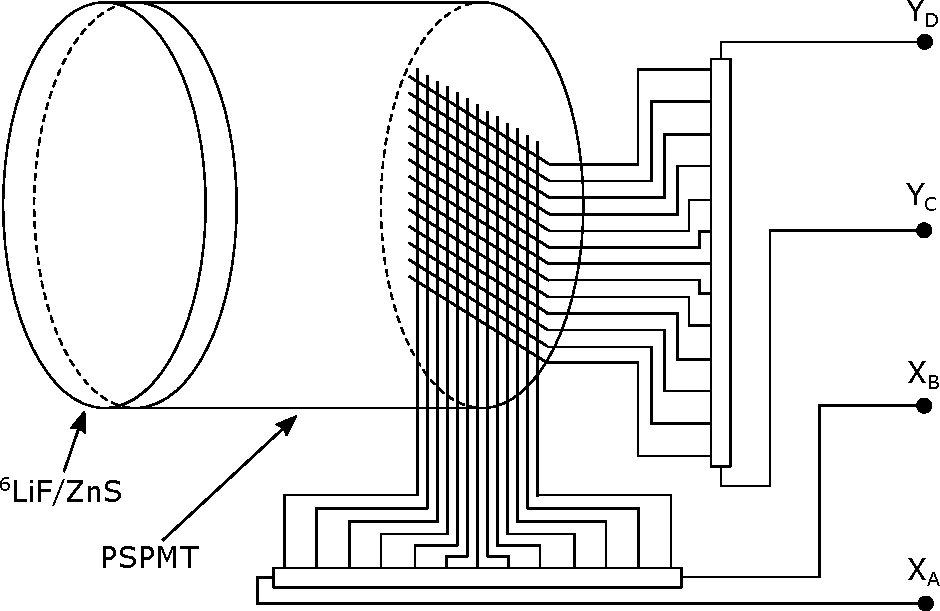
\includegraphics[width=6.5cm]{detector/detector_fig2.pdf}
\caption{RPMT写真}
\end{center}
\end{minipage}
\begin{minipage}{0.5\hsize}
\begin{center}
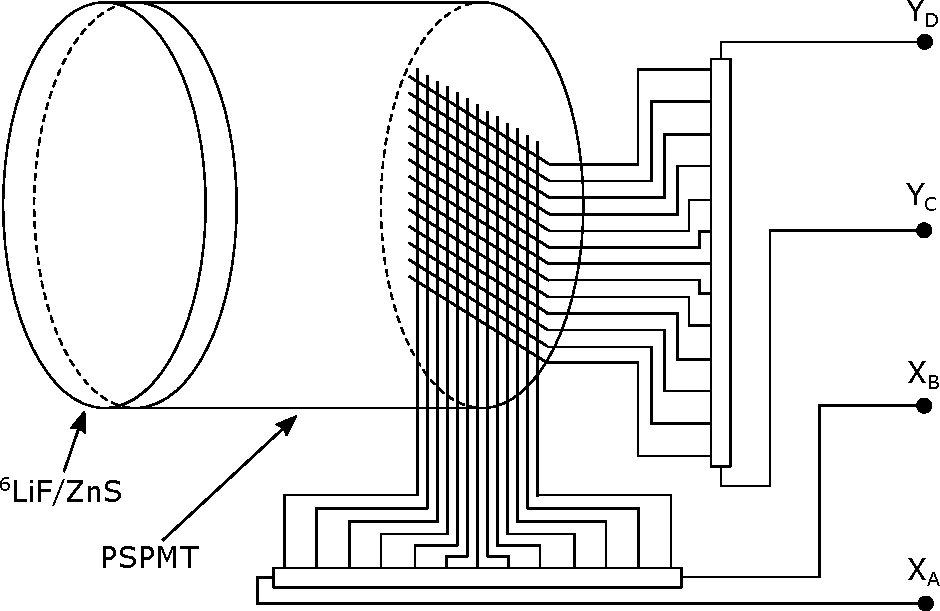
\includegraphics[width=6.5cm]{detector/detector_fig2.pdf}
\caption{RPMT模式図}
\end{center}
\end{minipage}\\
\begin{minipage}{0.5\hsize}
\begin{center}
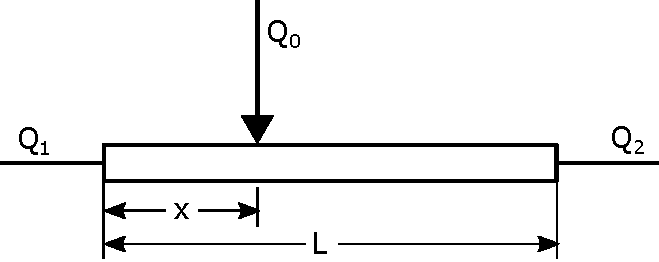
\includegraphics[width=6.5cm]{detector/detector_fig3.pdf}
\caption{電荷分割法}
\end{center}
\end{minipage}
\end{figure}






\begingroup
\def\imgwidth{5.5cm}

\section{位相シフタコイルによる干渉}
本実験である位相シフタコイルによる干渉について、実験手順、結果、解析の順に説明する。

\subsection{実験手順}
位相シフタコイルに流す電流を、0.0Aから3.3A, -0.3から-1.5までそれぞれ0.3A刻みで変え、各点10分程度測定した。

\subsection{実験結果}
干渉を見るためには、中性子のTOF(波長)を制限する必要がある。
どの波長を選ぶべきか判断するために、様々な波長での実験か結果をフィットして、最もビジビリティが高かった波長を採用することにする。

\paragraph{ビジビリティが最高となる波長}
上流フリッパーと下流フリッパーの反転率が1/2となるのは、予備実験からそれぞれ3.75Å, 3.56Åである。
その付近のいくつかの波長領域について、横軸を位相シフタに流した電流、縦軸をカウント数/LiMのカウント数で割ったものとしてプロットする。
実線は$-A\cos(Bx+C)+D$でフィットした結果を示している。
\begin{figure}[H]
\centering
\begin{minipage}{0.33\hsize}
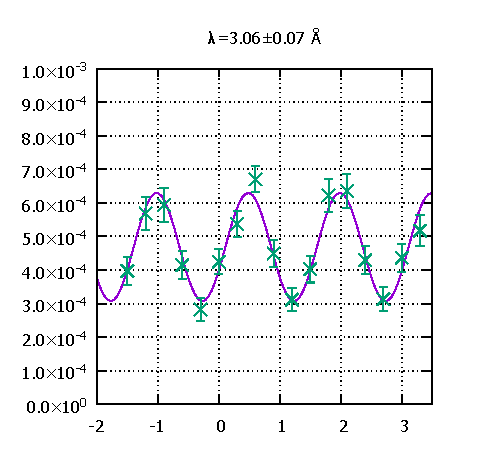
\includegraphics[width=\imgwidth]{phase_shifter/wl/wlf1.pdf}
\end{minipage}
\begin{minipage}{0.33\hsize}
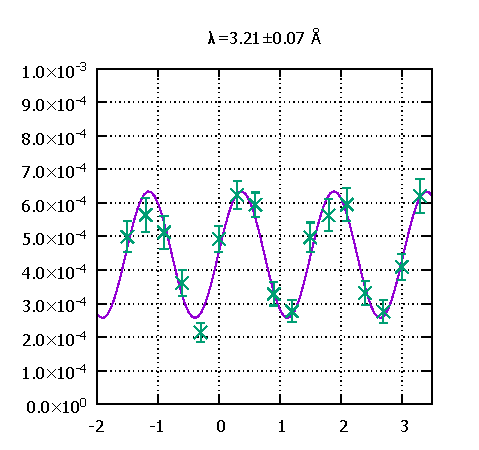
\includegraphics[width=\imgwidth]{phase_shifter/wl/wlf2.pdf}
\end{minipage}
\begin{minipage}{0.33\hsize}
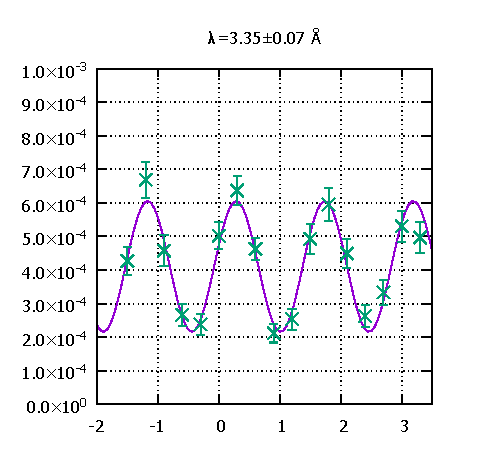
\includegraphics[width=\imgwidth]{phase_shifter/wl/wlf3.pdf}
\end{minipage}\\
\begin{minipage}{0.33\hsize}
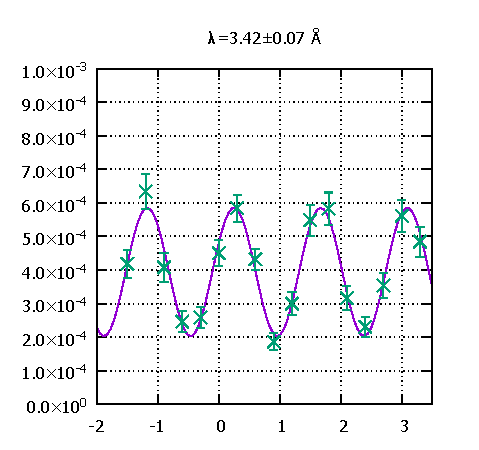
\includegraphics[width=\imgwidth]{phase_shifter/wl/wlf12.pdf}
\end{minipage}
\begin{minipage}{0.33\hsize}
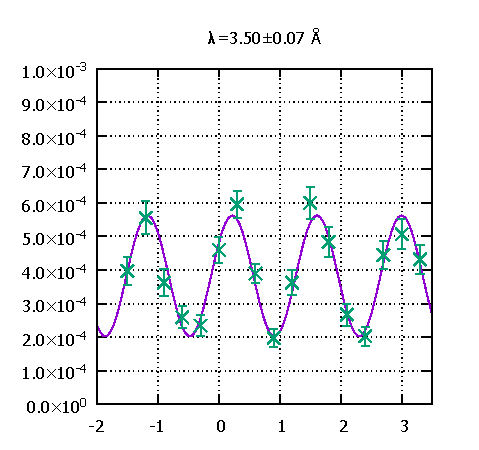
\includegraphics[width=\imgwidth]{phase_shifter/wl/wlf4.pdf}
\end{minipage}
\begin{minipage}{0.33\hsize}
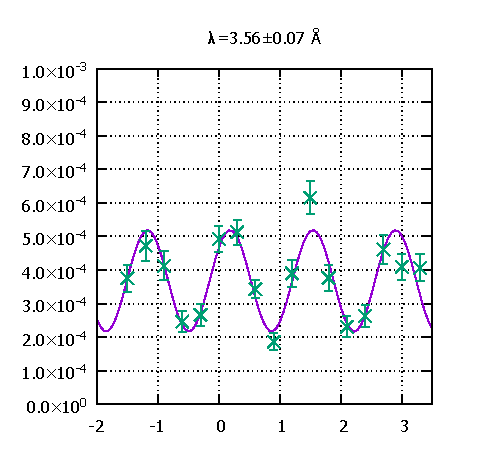
\includegraphics[width=\imgwidth]{phase_shifter/wl/wlf5.pdf}
\end{minipage}
\begin{minipage}{0.33\hsize}
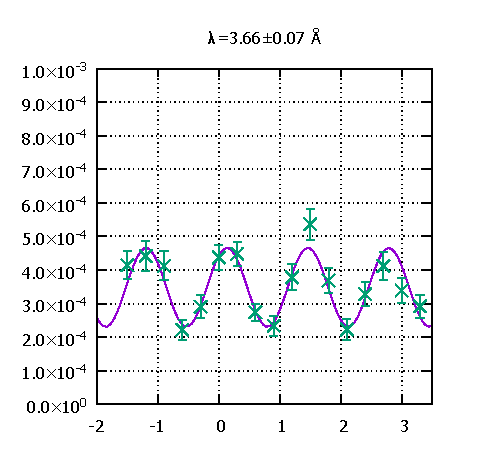
\includegraphics[width=\imgwidth]{phase_shifter/wl/wlf11.pdf}
\end{minipage}
\begin{minipage}{0.33\hsize}
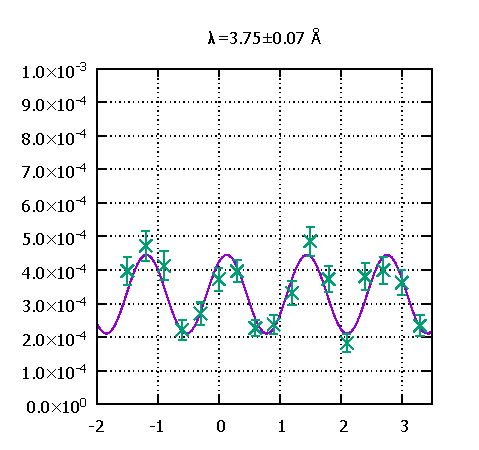
\includegraphics[width=\imgwidth]{phase_shifter/wl/wlf6.pdf}
\end{minipage}
\begin{minipage}{0.33\hsize}
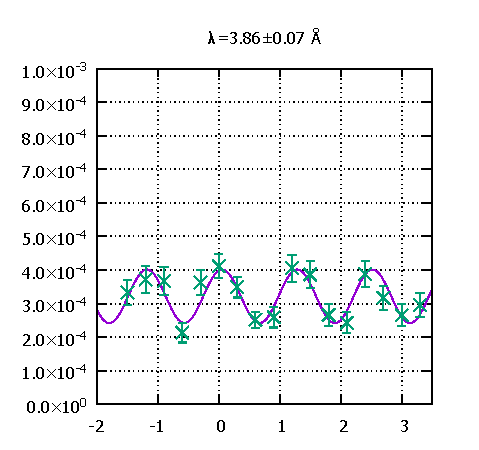
\includegraphics[width=\imgwidth]{phase_shifter/wl/wlf7.pdf}
\end{minipage}
\begin{minipage}{0.33\hsize}
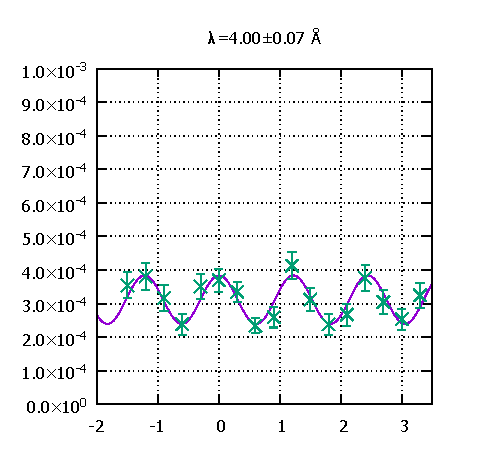
\includegraphics[width=\imgwidth]{phase_shifter/wl/wlf9.pdf}
\end{minipage}
\begin{minipage}{0.33\hsize}
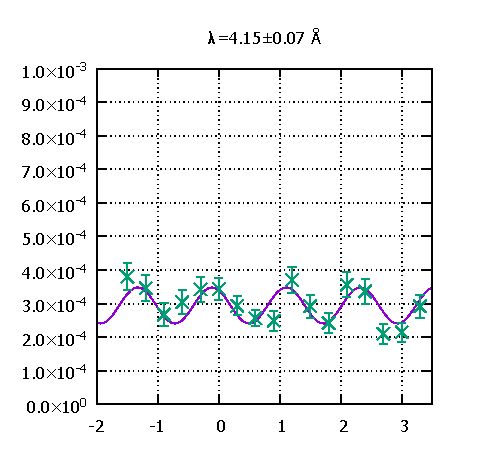
\includegraphics[width=\imgwidth]{phase_shifter/wl/wlf10.pdf}
\end{minipage}
\begin{minipage}{0.33\hsize}
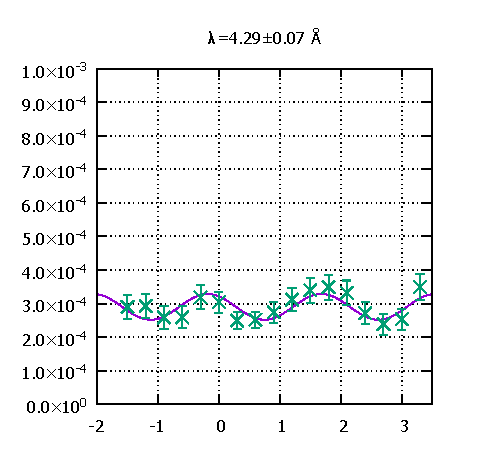
\includegraphics[width=\imgwidth]{phase_shifter/wl/wlf8.pdf}
\end{minipage}
\caption{各波長領域におけるカウント数/LiMカウント数。横軸は位相シフタコイルに流した電流。}
\end{figure}

フィット結果からビジビリティ$V\equiv A/D$を算出し、プロットすると以下のようになる:
\begin{figure}[H]
\centering
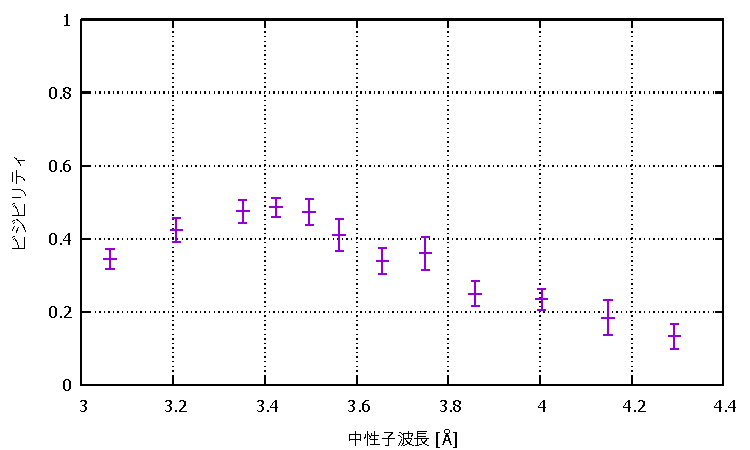
\includegraphics{phase_shifter/visibility.pdf}
\caption{波長ごとのビジビリティ。誤差はフィッティング誤差に由来する。}
\end{figure}

$\lambda=3.42\pm0.07$Åで最もビジビリティが高くなっていることがわかる。

\paragraph{最高ビジビリティとなる波長における結果}
$\lambda=3.42\pm0.07$Åにおける実験結果を以下に示す。
今後の解析はこの波長で行うことにする。
\begin{figure}[H]
\centering
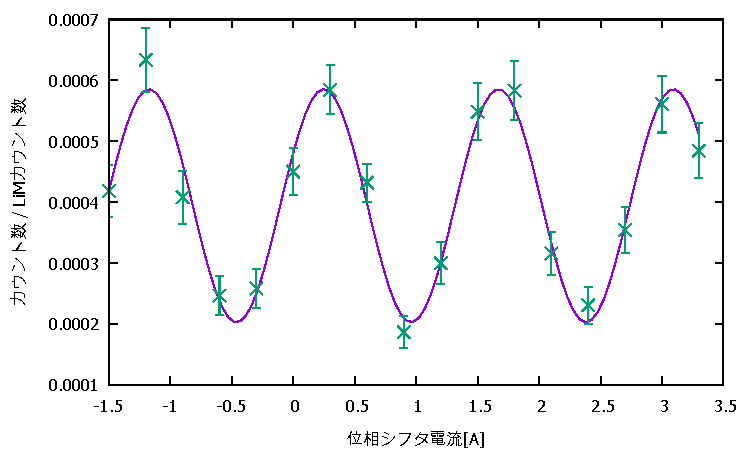
\includegraphics{phase_shifter/fit.pdf}
\caption{$\lambda=3.42\pm0.07$Åにおける実験結果とフィット。\label{ps_fitresult}}
\end{figure}

\subsection{解析}
\paragraph{理論値との対応}
図\ref{ps_fitresult}の縦軸はカウント数/LiMカウント数であり、これは理論値と直接対応する値ではない。
これを理論値と対応付けるために、$|\langle\uparrow|\uparrow\rangle|^2$に対応する、フリッパーをオフにしてスピンをフリップさせずに検出
した時のカウント数/LiMカウント数で割る必要がある。

$\lambda=3.42\pm0.07$Åにおける$|\langle\uparrow|\uparrow\rangle|^2$に対応するカウント数/LiMカウント数は、
$(6.73\pm0.53)\times10^{-4}$であった。この値で規格化した実験結果とフィット結果は以下の通りである:
\begin{figure}[H]
\centering
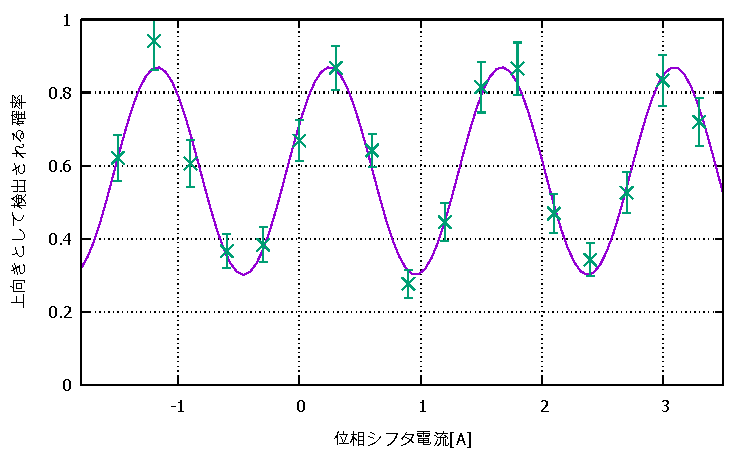
\includegraphics{phase_shifter/highest.pdf}
\end{figure}
\begin{table}[H]
\centering
\begin{tabular}{|r|r|}
\hline
$A$&$0.28\pm0.03$\\
\hline
$B$&$4.42\pm$0.04\\
\hline
$C$&$2.04\pm0.06$\\
\hline
$D$&$0.585\pm0.04$\\
\hline
\end{tabular}
\caption{フィット結果。フィット関数は$-A\cos(Bx+C)+D$}
\end{table}

\paragraph{理論値との比較}
理論式(\ref{theoretical})との比較を行う。
理論式
\begin{align}
|({\psi}_{Ⅶ}(x,t))_{+}|^2
=1-\cos^2\left({\omega}d'/v\right)\sin^2\left(\frac{2\omega_{r}}{v}d\right)\tag{\ref{theoretical}}
\end{align}
のうち、$\sin^2(2\omega_{r}/vd)$については、今$\pi/2$フリップ条件を満たしていることを仮定すれば1である。
従って、以下のように簡略化することができる:
\begin{align}
|({\psi}_{Ⅶ}(x,t))_{+}|^2=\frac{1}{2}\left(
1-\cos\frac{2{\omega}d'}{v}
\right)
\end{align}

$\omega$を電流に対応させることで、理論式の$B$は$4.34$となる。
以上より、理論式のパラメーターをまとめると以下のようになる:
\begin{table}[H]
\centering
\begin{tabular}{|r|r|}
\hline
$A$&$0.5$\\
\hline
$B$&$4.34$\\
\hline
$C$&$0$\\
\hline
$D$&$0.5$\\
\hline
\end{tabular}
\caption{フィット結果。フィット関数は$-A\cos(Bx+C)+D$}
\end{table}

角振動数$B$については$2\sigma$の精度で一致していることがわかる。振幅$A$、位相$C$、オフセット$D$にはずれが見られる。
すれの原因については、後により深く考察する。

\endgroup

\section{実験装置}
本節では実験において使用した装置を説明する。
\subsection{ガイド磁場コイル}
ガイド磁場コイルには二つの役割を持っている\\
1.実験装置全体に渡って中性子の量子化軸を定める\\
2.垂直方向に地磁気を無視できる程の大きさの磁場を一様に印加する\\
特に二つ目の役割は重要であり磁場の大きさが地磁気に比べて十分大きくないと地磁気によるスピンの反転が起きてしまうことになる。\\
また、磁場の一様性は中性子が通過する場所によって干渉条件が大きくずれないことを保証する。\\
実験ではガイド磁場コイルに5.5Aの電流を流し、ビーム軸上で磁場の強さは約12~13Gとなった。\\
なお電流を5.5A流すとガイド磁場コイルの温度が60$^\circ$C以上になる部分もあったため、3台の扇風機で空冷しながら実験を行った。
\begin{figure}[h]
\begin{center}
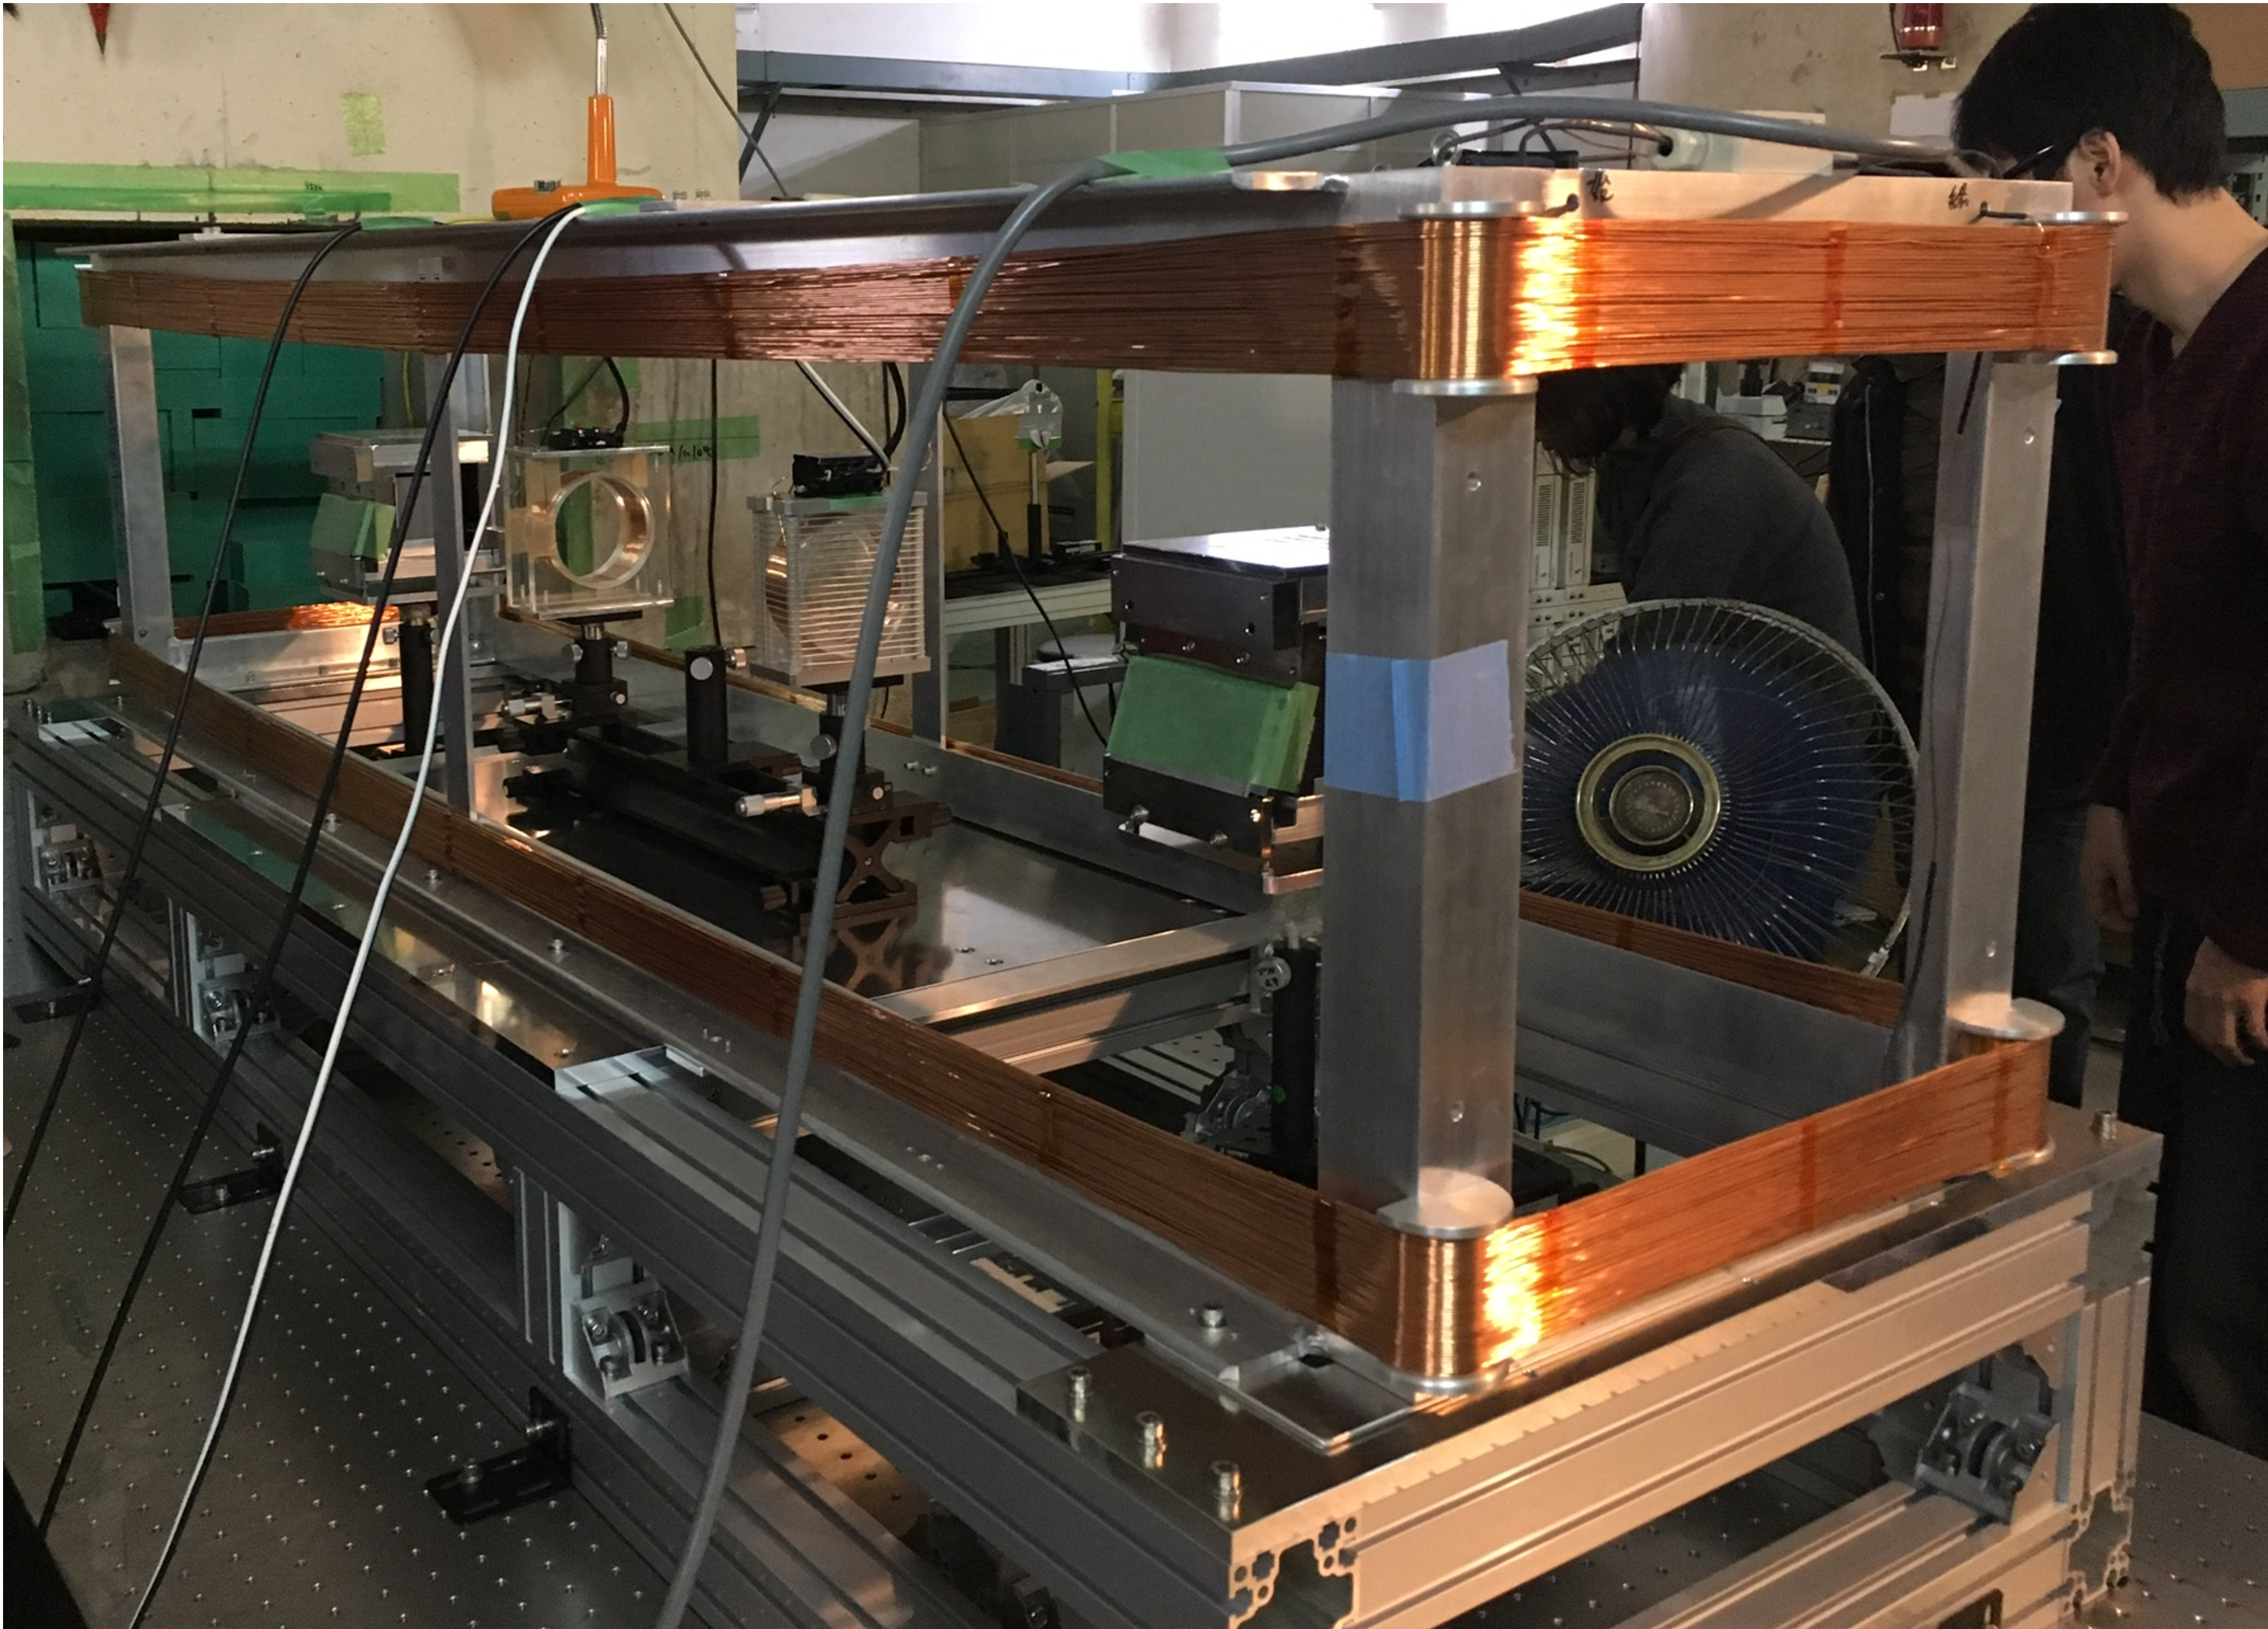
\includegraphics[width=8cm,height=5cm]{device/coilphoto.pdf}\caption{ガイド磁場コイル}
\end{center}
\end{figure}
\subsection{スピンフリッパ―}
スピンフリッパ―は入射中性子をスピン上向きと下向きの状態の重ね合わせにする役割を持つ。\\
装置としての構造は極めて単純で普通のソレノイドコイルである。コイルに高周波電流を流すことによって高周波磁場を作り出しスピンをフリップさせている。
\begin{figure}[H]
\begin{center}
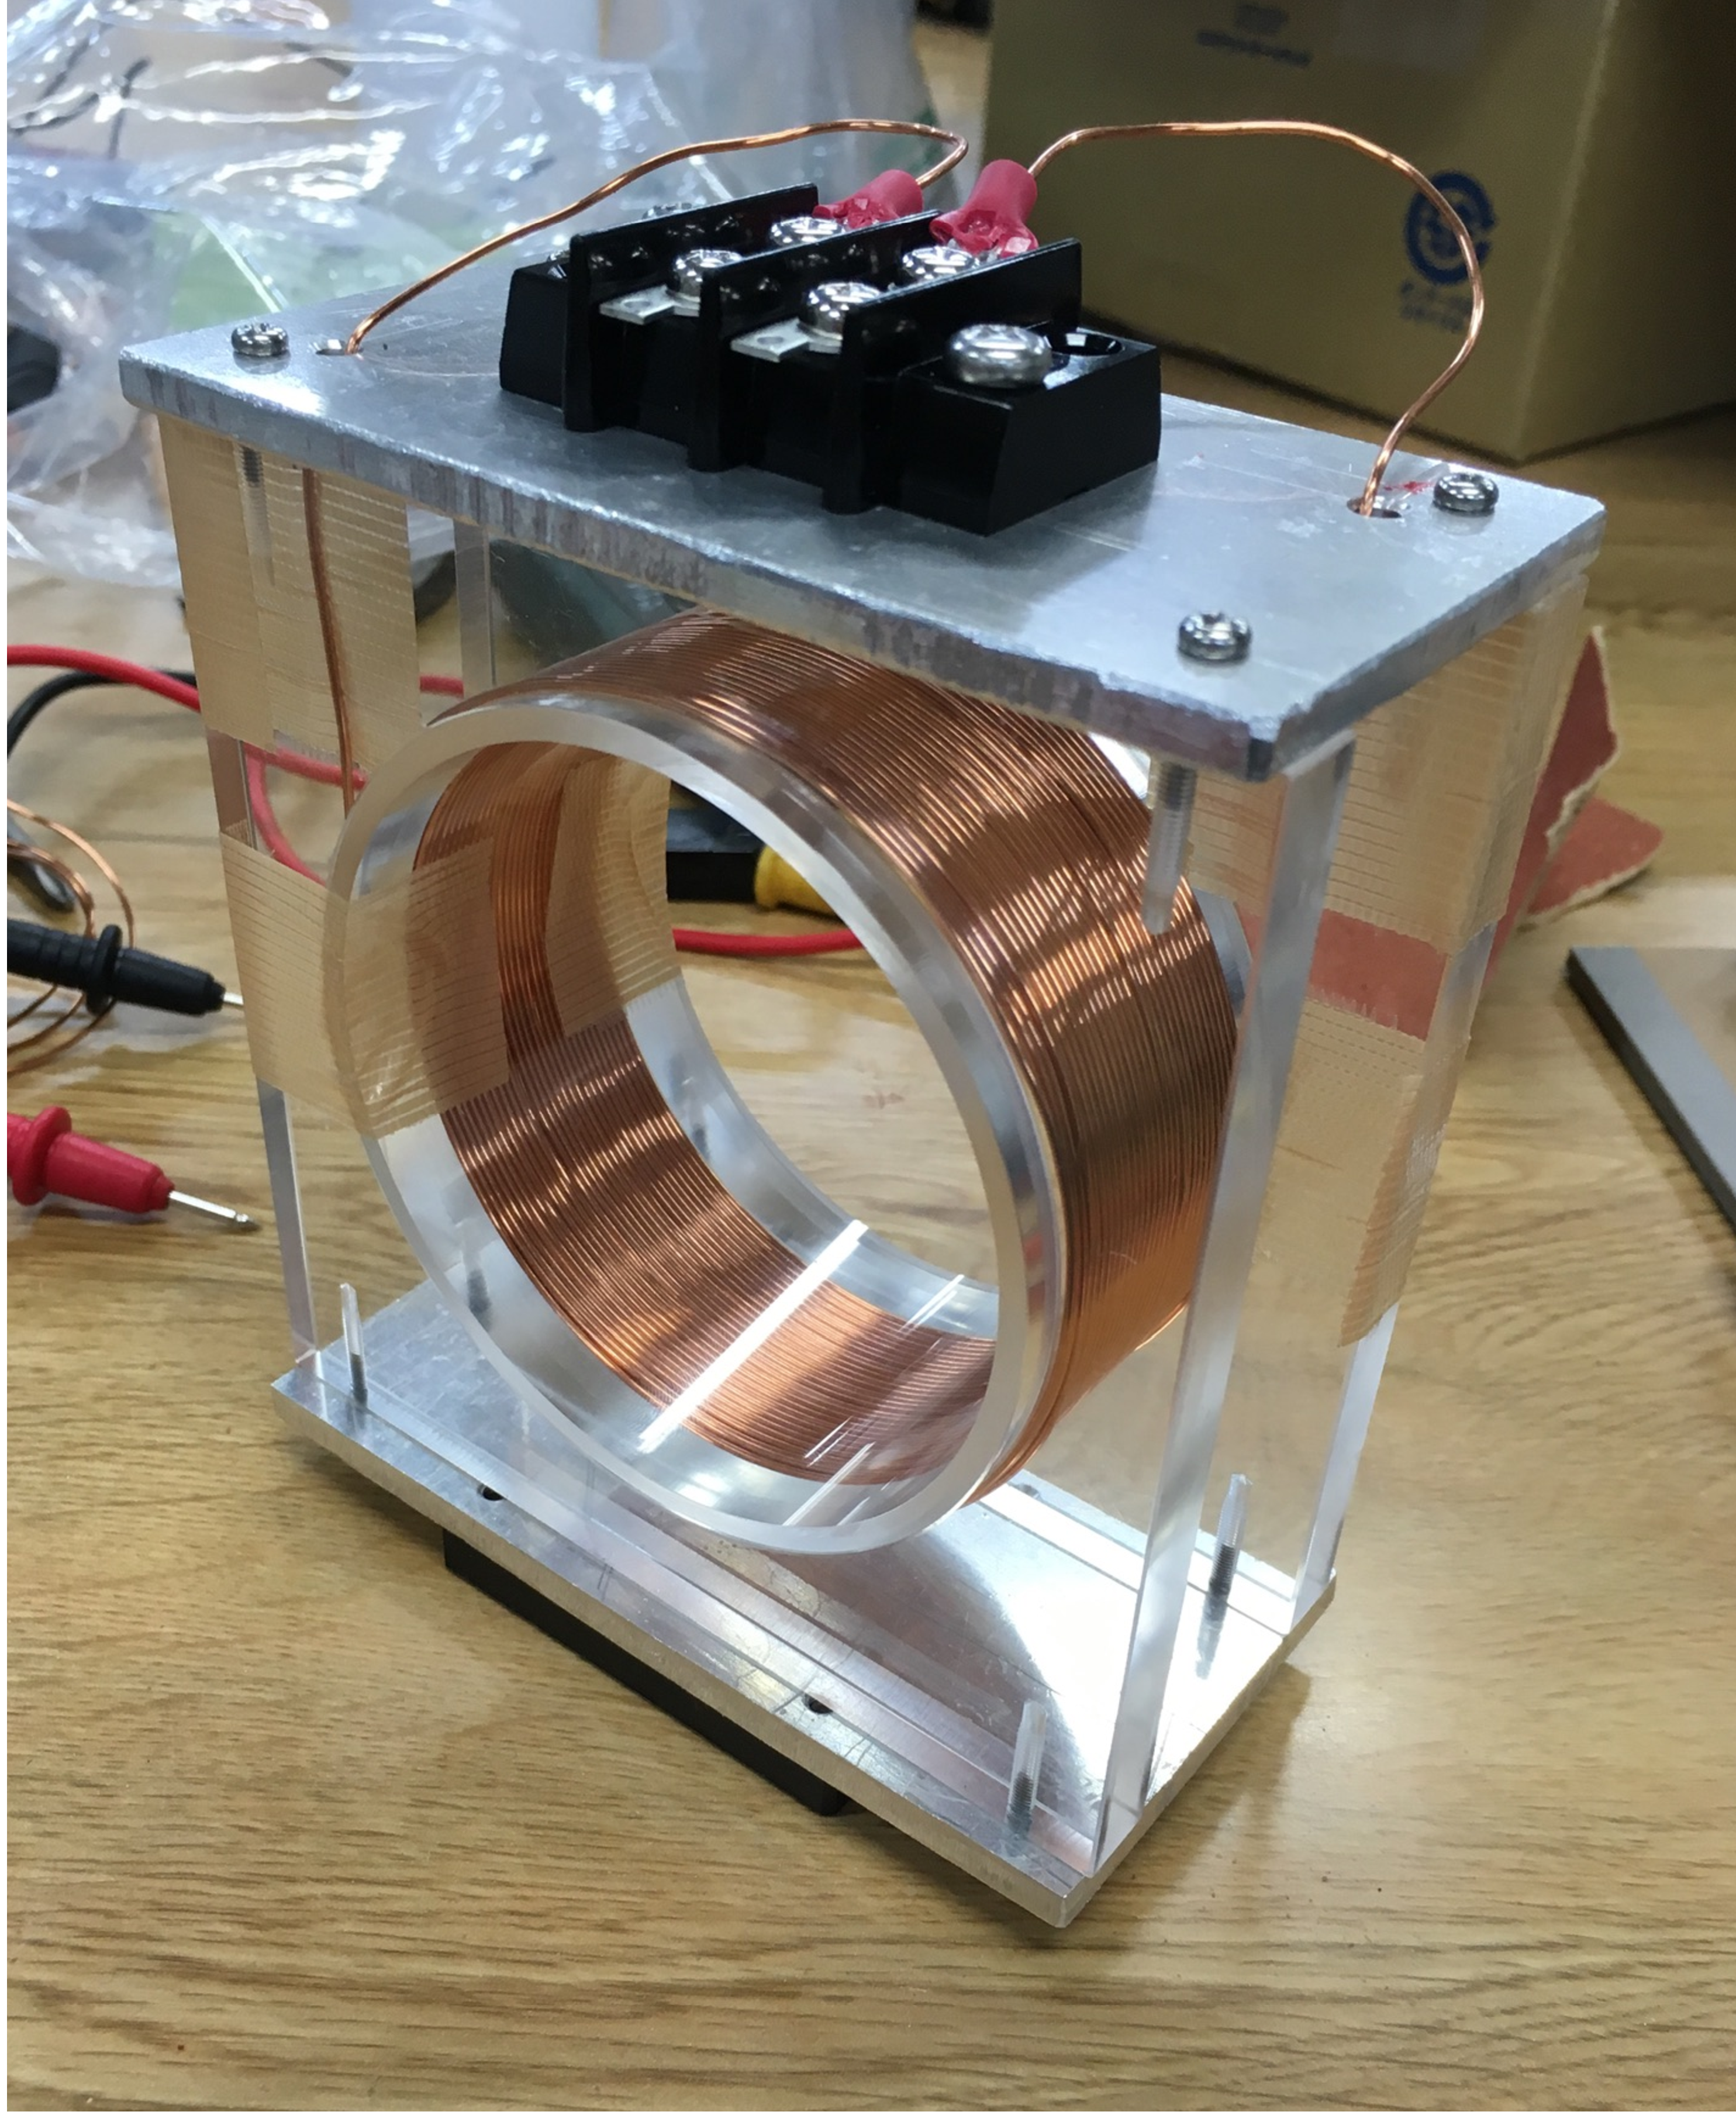
\includegraphics[width=5cm,height=6cm]{device/spinflipperphoto.pdf}\caption{自作したスピンフリッパ―}
\end{center}
\end{figure}
\subsection{位相シフタコイル}
位相シフタコイルの役割は垂直方向に磁場を作り出し、上向きスピンの中性子と下向きスピンの中性子それぞれに位相差を付けることである。\\
フリッパ―と同様にソレノイドコイルに定電流を流すことによって定磁場を作り出している。
\begin{figure}[H]
\begin{center}
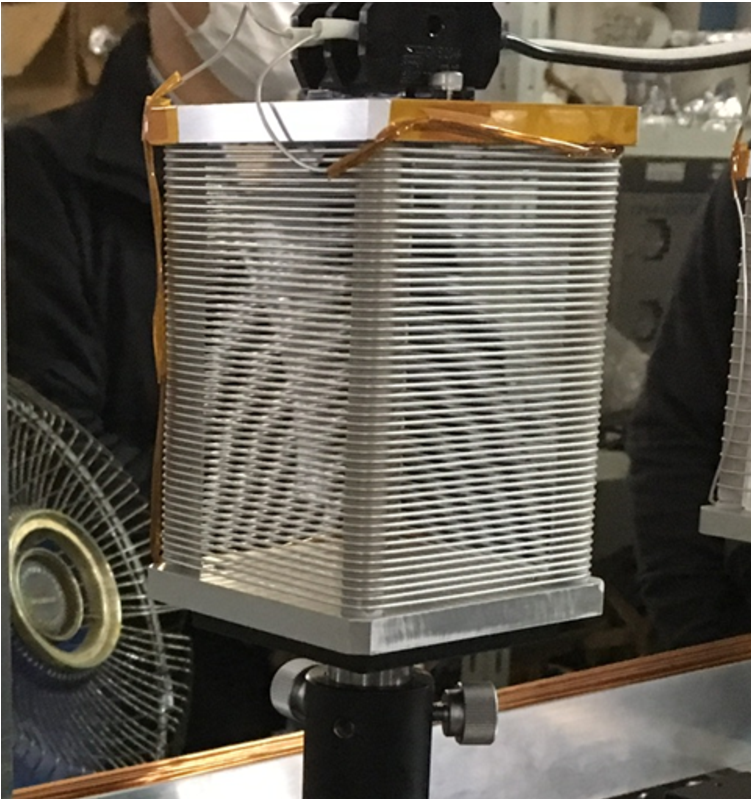
\includegraphics[width=5cm,height=6cm]{device/shifterphoto.pdf}\caption{位相シフタコイル}
\end{center}
\end{figure}
\bibliographystyle{jplain}
\bibliography{bibliography}
\end{document}
